\documentclass[12pt, titlepage]{article}
\usepackage{float}
\usepackage{booktabs}
\usepackage{tabularx}
\usepackage{hyperref}
\usepackage{graphicx}
\usepackage{titling}
\usepackage[utf8]{inputenc}
\usepackage{graphicx}
\usepackage{gensymb}
\usepackage{siunitx}
\graphicspath{{./images/}}
\usepackage{array}
\graphicspath{ {figures/} }

\hypersetup{
    colorlinks,
    citecolor=black,
    filecolor=black,
    linkcolor=blue,
    urlcolor=blue
}
\usepackage[round]{natbib}
\begin{document}

\title{
    MobiCharged\\Software Requirements Specification
    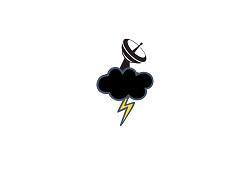
\includegraphics[width=9cm]{images/mobicharged.png} 
}
\author{Team Super Charged (No.33)
		\\ Nashit Mohammad - mohamn31
		\\ Eric Nguyen - nguyee13
		\\ Samuel De Haan - dehaas1
		\\ Eamon Earl - earle2
		\\ Mustafa Choueib - choueibm
}
    

\date{March 8th, 2023, Rev.1}


\maketitle

\pagenumbering{roman}
\tableofcontents
\listoffigures
\listoftables

\vspace{20pt}
\begin{center}
\begin{table}[H]
\caption{\bf Revision History}
    \begin{tabular}{p{2cm}p{3cm}p{2cm}p{6cm}}
    \hline
    \bf Author & \bf Date & \bf Version & \bf Description\\
    \hline
    All & October 5, 2022 & Rev 0 & Created First Draft of Document\\
    \hline
    Mustafa & November 9, 2022 & Rev 1 & Added New Functional and Non-Functional Requirements\\
    \hline
    Nashit & March 8, 2023 & Rev 1 & Added "User Characteristics" Under System Overview\\
    \hline
    Nashit & March 8, 2023 & Rev 1 & Added "Document Introduction" Under System Overview\\
    \hline
    Nashit & March 8, 2023 & Rev 1 & Updated "Background" Under System Overview\\
    \hline
    Nashit & March 9, 2023 & Rev 1 & Updated "Hardware System" Under Synopsis\\
    \hline
    Nashit & March 9, 2023 & Rev 1 & Added "Voltage Supply" Under Environmental Assumptions\\
    \hline
    Nashit & March 9, 2023 & Rev 1 & Updated Functional and Non-Functional Requirements Along With Corrected Naming Conventions\\
    \hline
    Nashit & March 10, 2023 & Rev 1 & Added "User Characteristics"\\
    \hline
    Nashit & March 10, 2023 & Rev 1 & Added Traceability Matrix\\
    \hline
    Mustafa & March 14, 2023 & Rev 1 & Provided Rationale for the Timeline\\
    \hline
    \end{tabular}
\end{table}
\end{center}

\newpage

\pagenumbering{arabic}

\section{System Overview}

\subsection{Naming Conventions and Terminology}

\begin{table}[H]
\caption{\bf Naming Conventions and Terminology}
\begin{tabular}{ |p{6cm}|p{8cm}|  } 
 \hline
\bf Word & \bf Definition/Context\\
 \hline
 FRs & Functional requirements that describe what the product is supposed to do\\
 \hline
NFRs & Non-functional requirements that describe qualities that product will have\\
 \hline
 Client & Client referring to the supervisor for which Project MobiCharged is conducted for; Mobilite Power\\
 \hline
GCs & Third party companies that acquire services by Mobilite-Power\\
  \hline
ECA & The Electrical Construction Association\\
\hline
Data Smoothing & The process of using old data as well as "future" data in order to predict designs\\
\hline
ML & "Machine Learning" algorithm\\
\hline
\end{tabular}
\end{table}

\subsection{Document Introduction}
In this document, the reader can expect to understand how the software intended for production will be expected to perform, as well as all the functionalities it is planned to accomplish for stakeholders. The document will cover a background/purpose, description of its stakeholders, and the project constraints. Following, it will outline both the software system as well as the hardware system at a high level. Moreover, the reader can expect to understand the project overview in which the types of operations will be highlighted, the system contexts and the system goals. In addition, the document will outline the system boundaries, operational concepts, assumptions, the requirements, the modes, and finally the plan of action. This document will follow the template provided by Dr. Smith from McMaster University labelled as "SRS" (Software Requirement Specification) as opposed to the "CA" (Commonality Analysis), which follows the idealogies from the Volere Template.

\subsection{Background}

Engineers are tasked with design in construction to exceed requirements without hindering safety. Safety is a topic that is never missed within the industry and is continuously being highlighted amongst designs; especially as Engineers are reminded of their moral obligations to society by their awarded rings upon graduation. 
\par
As a current process, the construction industry places sensors within concrete spaces to continuously test and/or monitor the integrity of buildings during as well as after construction. Ultimately however, these sensors run out of battery and are required to be re-charged.
\par
The industry still faces challenges when attempting to charge these sensors with the method of remote charging as the current products that satisfy remote charging abilities are yet to be optimized. There are a significant number of buildings being built in the GreaterToronto-Area, which is emphasized considering that 70\% of cranes within Canada are in just the GTA alone. To place innovation in the sub-field of safety within the industry, it is indeed a requirement to modernize the ability of producing efficient remote charging systems by having the design process optimized to provide the most effective results.
\par
The system-solution for this will be the development of MobiCharged. This system is separated into two separate components - the software for users as well as the hardware / prototype. 
\par
The software component of MobiCharged is a machine-learned system that will react to the input of users (in which the input will be the desired outputs / application requirements for the remote charging device) and provide the necessary results (these variables depending on the user inputs can be antenna types, layouts, wavelengths, phases, etc.)  in order to satisfy the user’s inputs such that they may proceed with producing the devices in a way that it is optimized. This software can be operated in any environment the user chooses such that it can be used in any computing system with sufficient speed, memory \& the required processors. 
\par
The hardware component of MobiCharged is a prototype to be developed for the purpose of demonstration as well as development for the software. This physical component will allow the system to be rooted to the core optimization problem in the real world, as it applies to real products. The physical system will allow placing absolute constraints and limitations into the software for optimal outputs in the software. In addition, this physical system can be implemented for an actual use-case in the field post-demonstrations. The environments in which these physical systems operate are typically from roof-tops and/or high-altitude locations with spacial capabilities to place arrays of these systems. These systems react to user inputted (remotely) data such as the location of the device required to be charged, so that it may orient itself in a manner optimal for that application. 

\subsection{Relevant Facts and Assumptions}
\begin{itemize}
    \item There is an assumption that the developers will eventually have access to enough processing power to conduct large quantities of simulations
    \item There is an assumption that the users operate the prototype system under "normal" conditions (which refer to the environment being between -20 degrees Celsius and 40 degrees Celcius, operation without the presence of intentional wave frequency inhibitors, and operation without the presence of significant magnetic fields
\end{itemize}

\subsection{User Characteristics}
The characteristics for which is recommended for the typical user to operate this project is of the following:\\
\begin{itemize}
    \item Familiar and confident in the ability of using a computer with WiFi capabilities with experience in operating desktop based applications
    \item Background knowledge in remote charging device's variables (which include but are not limited to phase shifts, frequency, amplitude, array type and array orientation).
    \item Background in electromagnetic and wave theory.
    \item Ages 14 and up for hardware system. Ages 16 and up for software system.
\end{itemize}


\subsection{The Stakeholders}

\subsubsection{The Client}
The client is Mobilite-Power.
\subsubsection{Other Stakeholders}
Other stakeholders for this project include Engineering Consultant Groups, General Contractors and Building Maintenance Teams.
\subsection{Mandated Constraints}

\subsubsection{Budget Constraints}

The project has a budgetary constraint of \$750

\subsubsection{Schedule Constraints}

The system must be completed by April 8th, 2023.

\section{Synopsis}
\subsection{Software System}
The purpose of the software system, MobiCharged, is a machine learning algorithm that will be used by the client and other stakeholders to optimize the design process required to effectively and efficiently produce the most viable remote charging system. In doing so, this will negate the current process of manually conducting simulations (that requires lengthy computerized numerical calculations), ultimately minimizing cost, manual labor, and the time necessary to produce the required results. 
\par
This system will provide users with the optimal configuration of a remote charging device based on the desired output, encrypt data protecting users when producing design results and use data smoothing to ensure the accuracy of the system in a time efficient manner.

\subsection{Hardware System}
The purpose of the hardware system is to root our algorithms optimization in the real world environment. The production of a physical model will assist in the determination of the absolute boundaries that can be fed into the machine learning algorithm. Variable parameter ranges will be able to be derived from the physical model to determine the magnitude to which the boundaries can be pushed within the simulation. 
\par
The physical system provides a secondary purpose in the form of data collection and verification. In order to increase the breadth of data that we can feed into the algorithm, we must determine the degree of computational error within the simulation results. A physical model will aid in determining this range and lead to further optimization through the machine learning algorithm. 
\par
To effectively meet the constraints of this project, the hardware system will be produced as a means of simulating a remote charging device as opposed to creating a real physical one (due to time \& budget constraints). As such, Team MobiCharged intends to create a physical simulation system that displays the fundamental concepts of remote charging devices by creating a 3D "levitator" capable of levitating particles through the means of electromagnetic waves. This "levitator" will encapsulate the ideas behind remote charging devices while simultaneously be used for demonstration purposes. The team intends to attach a sensor to the system such that real data can be retrieved from the hardware components and be fed into the software system as described above. As a potential back-up due to unforeseen circumstances, the hardware system at the very least can be applied as a means demonstrations and classes.   

\section{Project Overview}
\subsection{Normal Operation}
This application is to be used by the client to reduce overhead costs associated with developing remote charging devices. The company will be able to use this system on their computers with ease. By using this system, the client will be able to minimize the cost, time, and labor required to determine the optimal configuration necessary for remote charging devices. This will make their operations more efficient.

\subsection{Behaviour Overview}
This system will continuously learn and develop without an operator. However, the ultimate output of the system will be event based, thus, requiring the user to initiate operations. The user will be required to provide the necessary input, in which the machine learning algorithm will return the optimal configuration for a remote charging device, encrypt the provided output, and store the optimal data into a database for data smoothing. When the system is not in use, it will be running simulations automatically to continuously refine its ability to produce accurate optimal results.

\subsection{Undesired Event Handling}
Undesired event handling is critical to ensuring that, even in unintended circumstances, the system can safely revert to a desired state. Thus, the system should ensure that in the event of an error or fault, it has a fail-safe state to transition to. This fail-safe state will ensure that there are no corruptions in data, the system itself, or extensive damages caused.



\section{System Contexts}

\subsection{Preliminary System Contexts}
The system will interact with pre-existing matlab simulation programs, purely at the simulations’ start and end points, where the program will pull data from completed simulations and push parameters to run new ones. In the early stages of the product life cycle, it will mainly be pulling the completed simulation data, and feeding it into the deep learning algorithm in order to train it and give it some experience with optimal solutions. This will require integration with large databases in order to record this data. 
\par
Once the core program / deep learning algorithm has been trained to some satisfying degree, the context will expand to include the second half of the cyclical integration with the pre-existing simulation software; it will now take charge of running new simulations that push the boundaries of its current knowledge base. This is in order to take full advantage of free processing power, such that the simulations are always being run, and the deep learner is constantly being trained. This may require interfacing with an additional software module in order to schedule data coming in to be processed, and outward data to be procured. 
\par
Later in the life cycle of the program, we will be either integrating with the client's current remote desktop server (used to run the simulations remotely), or develop our own, where the specifics of this contextual decision will depend on the availability of their server at this time. The goal would be to integrate our program with the server such that our deep learner would be able to access the data from any simulation run, and not just those on the local devices of our team's, which also implies that the team plans on having these simulations able to be run on multiple different devices at the same time, eventually adding further scheduling and concurrency constraints to our learner-server pair. 
\par
Evidently, our context shifts and expands multiple times throughout the development lifecycle, as we wish to integrate with and expand upon pre-existing software in multiple areas of the design. The following context diagrams give an idea of this development, with each diagram associated, in order, with the above paragraphs. The components will be briefly described alongside each diagram for clarity.
\newpage


\begin{figure}[h]
    \centering
    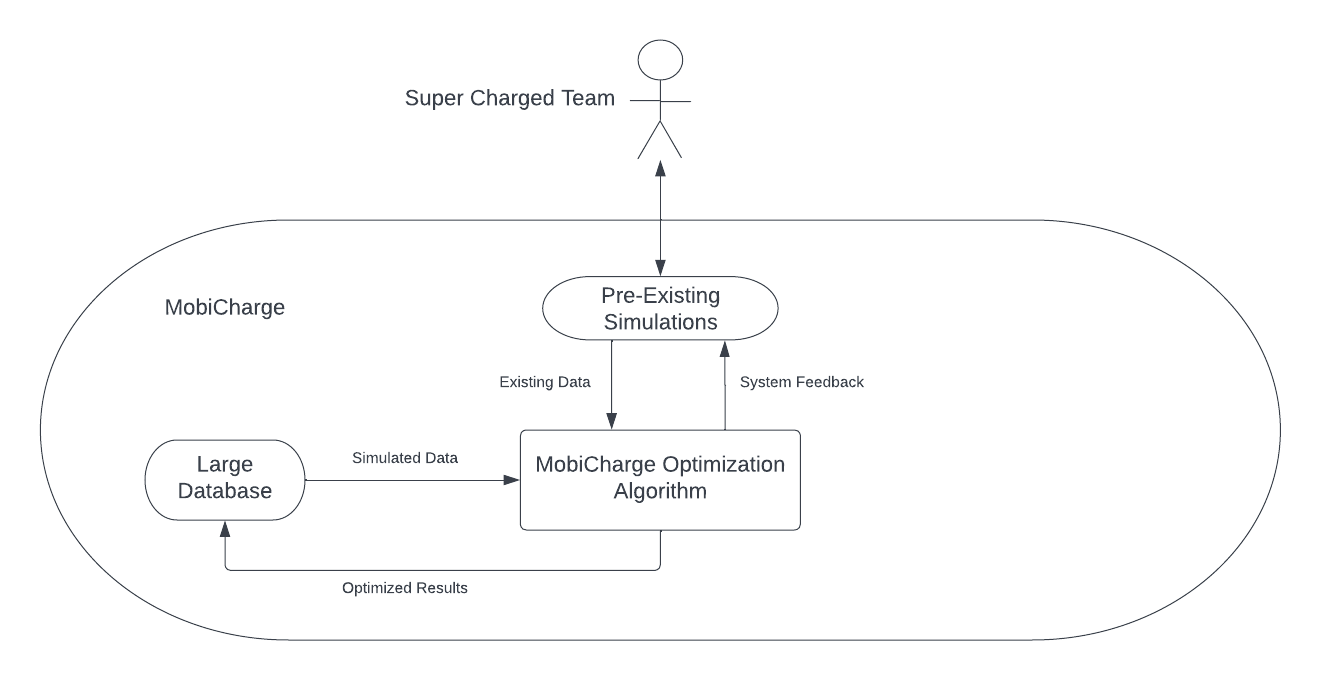
\includegraphics[width=15cm]{images/context0.png}
    \caption[Prelim System Contexts 1]{First stage of preliminary system context.}
    \label{fig:figure1}
\end{figure}

The external entity, the Super Charged team; the team of developers for the system, will begin to train the MobiCharged software system using pre-existing simulation data. The simulations that are optimized by the system will then be stored into a large database for further use by the system. As shown by figure 1.
\par
\newpage
\begin{figure}[h]
    \centering
    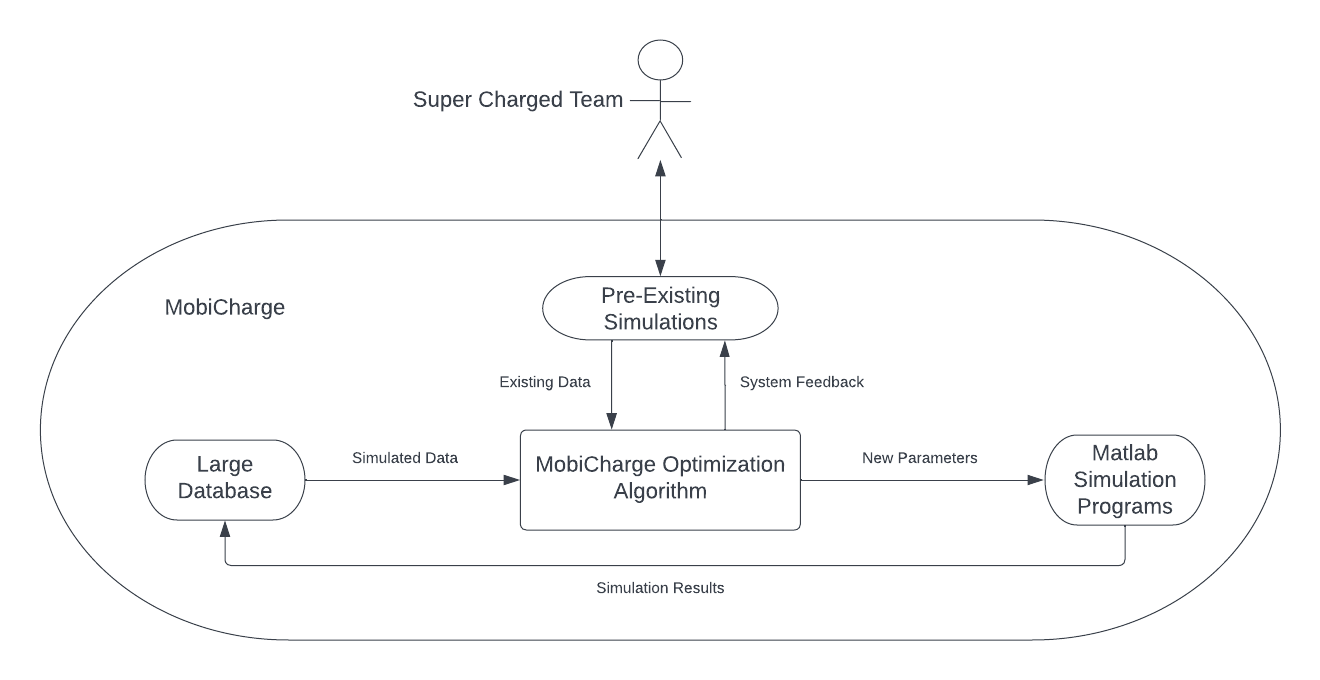
\includegraphics[width=15cm]{images/context1.png}
    \caption[Prelim System Contexts 2]{Second stage of the preliminary system context.}
    \label{fig:figure2}
\end{figure}
As shown in figure 2, the external entity, the Super Charged team, will then integrate the optimization algorithm with pre-existing simulation software. This will allow the system to conduct simulations automatically, furthering the knowledge base of the system. 

\newpage
\begin{figure}[h]
    \centering
    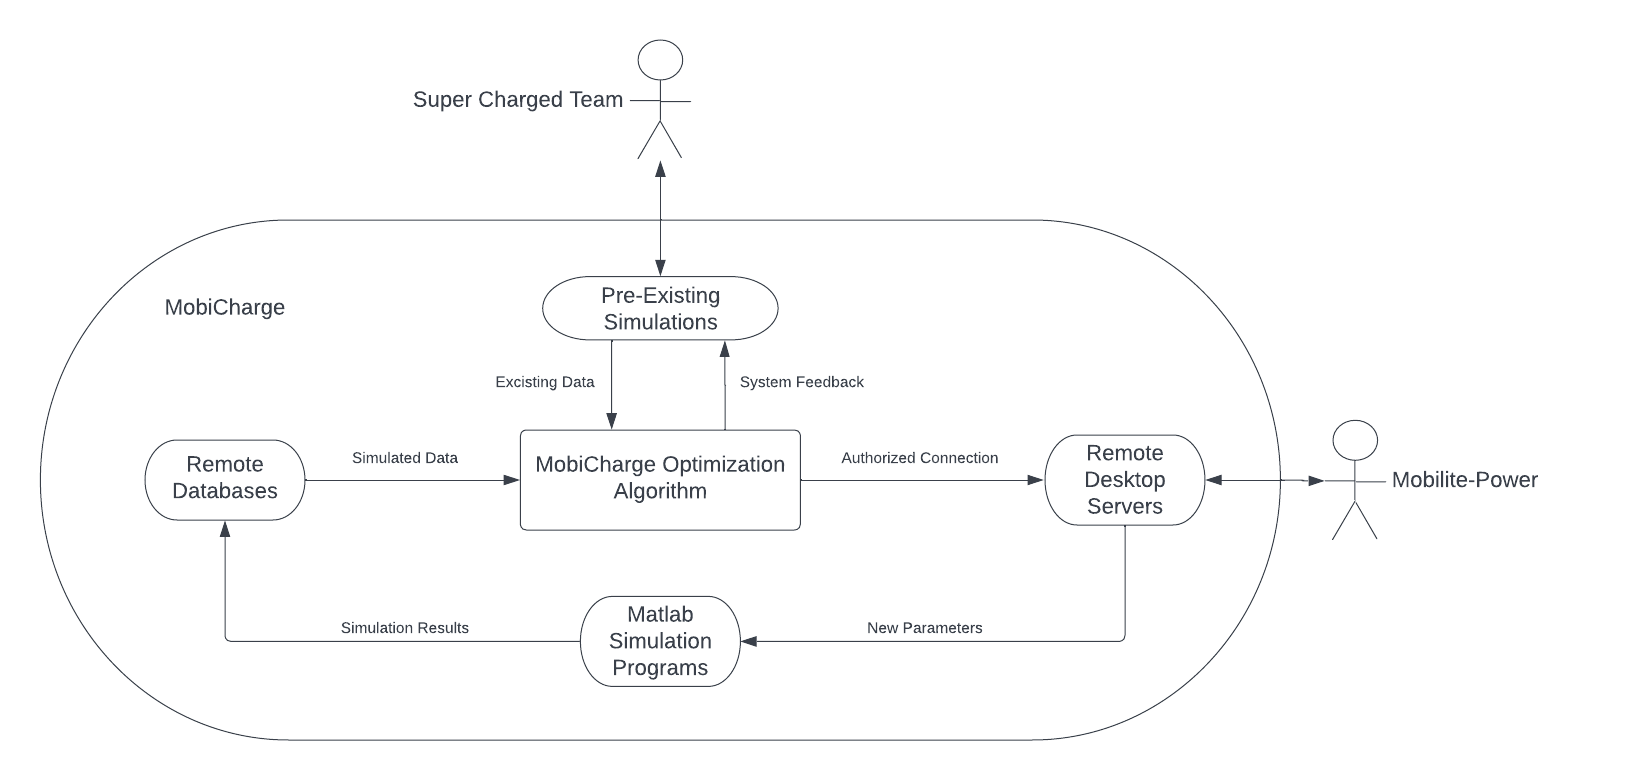
\includegraphics[width=15cm]{images/context2.png}
    \caption[Prelim System Contexts 3]{Final stage of the preliminary system context.}
    \label{fig:figure3}
\end{figure}
The last stage of the preliminary system context is as shown in figure 3. The external entities are the Super Charged team, as well as the Mobilite-Power company. Mobilite-Power is the external entity which oversees the data acquired from the simulations and provides the machines with the necessary configurations for the remote charging devices. Mobilite-Power will provide access to remote desktop servers, which the Super Charged team will then integrate into the system, allowing for more simulations to be accessed by the system. This will further train the system, increasing the accuracy of the optimizations produced by the system.


\newpage
\subsection{Server Integrated System Context}

\begin{figure}[h]
    \centering
    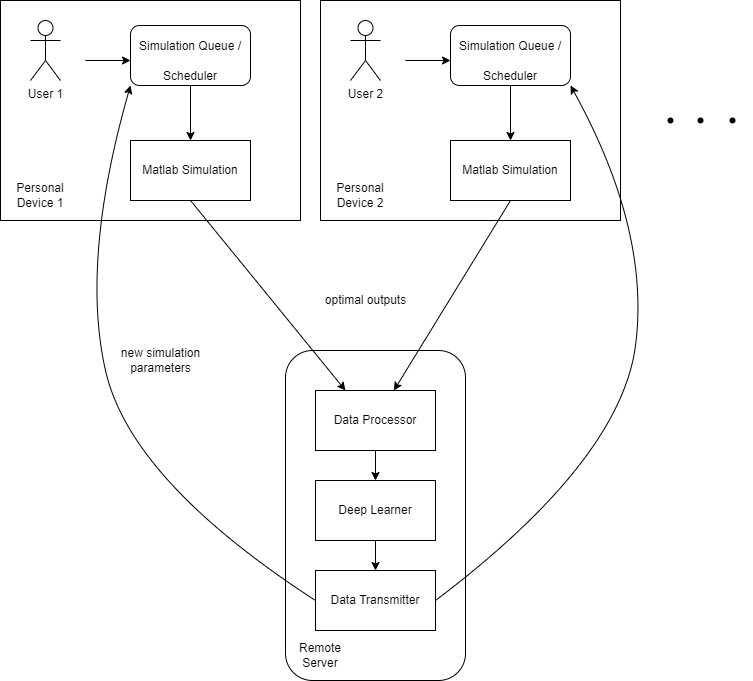
\includegraphics[width=15cm]{images/server_system.png}
    \caption[Server-Int System Contexts 1]{System context integrated with servers.}
    \label{fig:figure4}
\end{figure}

The divide between personal devices and the server will likely be structured as shown above, where the deep learner exists as a part of a central server, and the core computations of the simulations can be done on local machines. This allows the server to remain relatively low fidelity for the time being, where its core computations are the algorithms of the deep learner itself. The data processor and transmitters will handle concurrency and syncing with local devices. This obviously requires cooperation and coordination of these local devices, and this may not be ideal for commercial use. The goal is to prioritize data throughput in the development stage, leaving the simulations relatively untouched and implementing enough modularity such that the server can be formalized and protected with more elegance down the line, and integrated with higher-fidelity computing devices.

\subsection{Deployed System Context}
Once the system has been sufficiently trained and developed, it will be deployed for commercial use. However, the software system will continuously be trained and the throughput will continue to be refined. In a commercial setting, the system will interact with the client, who will feed the desired output to the system, and the system will produce the optimal configuration for a remote charging device. This data will be exported to the client's production team once the system has encrypted the data. The system will also be able to decrypt the data following the export, and retrain the system with the optimized results. Lastly, the optimized data will be stored in a database to repeatedly enhance the accuracy of the system.
\newpage

\begin{figure}[h]
    \centering
    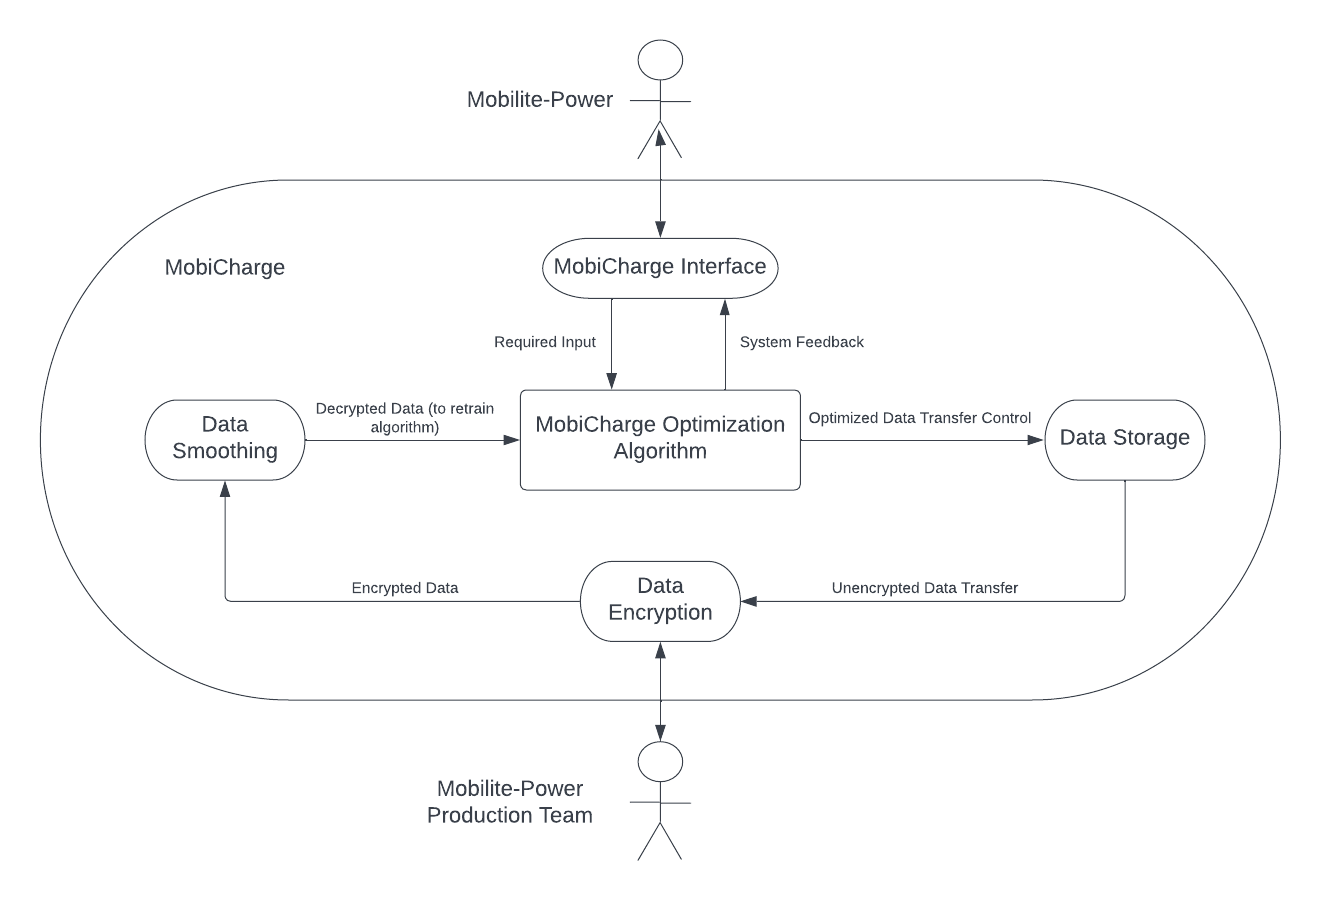
\includegraphics[width=15cm]{images/context3.png}
    \caption[Deployed System Contexts 1]{Stage of the deployed system context.}
    \label{fig:figure5}
\end{figure}
As shown in figure 5, the external entities acting on the system are the Mobilite-Power group responsible for determining the optimal configuration for the remote charging device, and the Mobilite-Power production team responsible for building the remote charging device. The Mobilite-Power entity will access the system and provide the desired output of the remote charging device. The system will then produce the optimal configuration and provide that configuration to the production team in an encrypted manner. 

\section{System Goals}
Below are the listed summarized general goals of the system. For further information on the goals, please refer to the document "CapstoneProblemStatement\_Goals".

\begin{itemize}
    \item Goal 1: Machine Learning Optimization Study
    \begin{itemize}
        \item Origin: Client - Mobilite Power.
        \item Origin Date: Semptember 9th, 2022.
        \item Author: Eamon Earl.
        \item Priority: High.
        \item Stakeholders: Client, Customers, Consultant Engineers, General Contractors, Builders.
        \item Stability: Strong - goal not likely to change
        \item Schedule Date: March 20th, 2023.
    \end{itemize}
    \item Goal 2: Data Collection
    \begin{itemize}
        \item Origin: Individual Developers Associated with MobiCharged.
        \item Origin Date: Semptember 12th, 2022.
        \item Author: Nashit Mohammad.
        \item Priority: High.
        \item Stakeholders: Client, Customers, Consultant Engineers, General Contractors, Builders.
        \item Stability: Strong - goal not likely to change
        \item Schedule Date: November 9th, 2022.
    \end{itemize}
    \item Goal 3: Robustness in Software
    \begin{itemize}
        \item Origin: Individual Developers Associated with MobiCharged.
        \item Origin Date: Semptember 13th, 2022.
        \item Author: Mustafa Choueib.
        \item Priority: Mid.
        \item Stakeholders: Client, Customers, Consultant Engineers.
        \item Stability: Stable / Mid-Strength.
        \item Schedule Date: March 1st, 2023.
    \end{itemize}
    \item Goal 4: Software Time in Completion
    \begin{itemize}
        \item Origin: Client - Mobilite Power.
        \item Origin Date: Semptember 13th, 2022.
        \item Author: Eric Nguyen.
        \item Priority: High.
        \item Stakeholders: Client, Customers, Consultant Engineers, General Contractors, Builders.
        \item Stability: Stable / Mid-Strength.
        \item Schedule Date: December 12th, 2022.
    \end{itemize}
    \item Goal 5: Prototype is Resilient to External Environment Conditions
    \begin{itemize}
        \item Origin: Individual Developers Associated with MobiCharged \& ECA Regulations.
        \item Origin Date: Semptember 13th, 2022.
        \item Author: Sam De Haan.
        \item Priority: Low.
        \item Stakeholders: Client, Customers, Consultant Engineers, General Contractors, Builders, Residents in Nearby Buildings, Local Wildlife.
        \item Stability: Weak - can change depending on constraints.
        \item Schedule Date: March 20th, 2023.
    \end{itemize}
    \item Goal 6: Ease of Use
    \begin{itemize}
        \item Origin: Client - Mobilite Power.
        \item Origin Date: Semptember 9th, 2022.
        \item Author: Nashit Mohammad.
        \item Priority: Low.
        \item Stakeholders: Client, Customers, Maintenance Teams.
        \item Stability: Weak - can change depending on constraints.
        \item Schedule Date: March 20th, 2023.
    \end{itemize}

\end{itemize}


\section{System Boundary}
\subsection{Preliminary Set of Monitored \& Controlled Variables}
\begin{table}[H]
\caption{\bf Monitored \& Controlled Variables}
    \begin{tabular}{|p{4cm}|p{3cm}|p{7cm}|}
         \hline
         \bf Name & \bf Type & \bf Physical Interpretation\\
         \hline
         Charging Device's Range & Monitored & Maximum reach of for device charging.\\
         \hline
         Device's Lower Allowed Charge & Monitored & Minimum level of charge allowed in device before charging is required.\\
         \hline
         Device's Upper Desired Charge & Monitored & Level of charge desired in drive to be charged.\\
         \hline
         Wireless Charging Control & Controlled & \\
         \hline
         Displayed Device Charge & Controlled & \\
         \hline
         Current Supply & Controlled & Value of current supplied to charging device.\\
         \hline
         Charging Device Frequency & Controlled & Frequency used by charging device.\\
         \hline
         Phase Shift & Controlled & Phase shift used by charging device.\\
         \hline
    \end{tabular}
\end{table}


\subsection{Environment Variables}
\begin{table}[H]
\caption{\bf Environment Variables}
\begin{tabular}{ |p{4cm}|p{3cm}|p{7cm}|} 
 \hline
\bf Name & \bf Type & \bf Physical Interpretation\\
 \hline
 Position of Device to be Charged & Environmental & Relative distance from device to be charged to charging device.\\
 \hline
 Density of Medium & Environmental & Density of medium which charging device must charge through.\\
\hline
\end{tabular}
\end{table}


\section{Operational Concepts}

\begin{itemize}
    \item Use case S.1.1: Normal Operation of MobiCharged
    \item This use case described the normal operation of the software system, MobiCharged, by Mobilite-Power.
    \item \underline{Related System Goals:} Goal 1
    \item \underline{Primary Actor:} Mobilite-Power
    \item \underline{Precondition:}
    \begin{itemize}
        \item Mobilite-Power receives purchase order for remote charging device.
        \item Desired output is clearly indicated.
    \end{itemize}
    \item \underline{Postcondition:}
    \begin{itemize}
        \item Optimal configuration for remote charging device is procured.
        \item Relevant data is processed and stored by the system.
    \end{itemize}
    \item \underline{Main Success Scenario:}
    \begin{enumerate}
        \item User accesses the system through the interface.
        \item User provides the necessary input to the system.
        \item System begins producing the optimal output in the normal mode of operation.
        \item System determines the optimal output based on the given input.
        \item System transfers the optimized data to the data storage.
        \item The system encrypts the data and exports the output to the user.
        \item The system decrypts that data once again.
        \item The system retrains itself using the optimized decrypted data.
        \item System returns to its normalized idle state.
    \end{enumerate}
\end{itemize}



\section{Environmental Assumptions}
The following section will document the assumptions made on the system environment. This will define each variable within the system environment and provide an indication for each that is required for proper operation.

\begin{center}
\begin{tabular}{|p{3cm}|p{1cm}|p{1cm}|p{2cm}|p{1cm}|p{6cm}|}
\hline
\underline{Name} & \underline{Type} & \underline{Range} & \underline{Precision} & \underline{Units} & \underline{Physical Interpretation}\\[5pt]
\hline
Charging Device Range & Real & 0-5 & $\pm0.1$ & m & Maximum reach of for device charging.\\
\hline
\end{tabular}
\end{center}


In order for the charging device to work, the device to be charged must be within range. This adds a limit on the area of operation. Range was assumed based on standard operating conditions and limits of technology.

\begin{center}
\begin{tabular}{|p{3cm}|p{1cm}|p{1cm}|p{2cm}|p{1cm}|p{6cm}|}
\hline
\underline{Name} & \underline{Type} & \underline{Range} & \underline{Precision} & \underline{Units} & \underline{Physical Interpretation}\\[5pt]
\hline
Device's Lower Allowed Charge & Real & 0-99 & $\pm0.1$ & \% & Minimum level of charge allowed in device before charging is required.\\
\hline
\end{tabular}
\end{center}

The rationale behind these assumptions are based on clients' needs. A device may require differing levels of charge for proper operation. 

\begin{center}
\begin{tabular}{|p{3cm}|p{1cm}|p{1cm}|p{2cm}|p{1cm}|p{6cm}|}
\hline
\underline{Name} & \underline{Type} & \underline{Range} & \underline{Precision} & \underline{Units} & \underline{Physical Interpretation}\\[5pt]
\hline
Device's Upper Desired Charge & Real & 1-100 & $\pm0.1$ & \% & Level of charge desired in drive to be charged\\
\hline
\end{tabular}
\end{center}

A device may require differing levels of maximum charge depending on the clients’ needs.

\begin{center}
\begin{tabular}{|p{3cm}|p{1cm}|p{1cm}|p{2cm}|p{1cm}|p{6cm}|}
\hline
\underline{Name} & \underline{Type} & \underline{Range} & \underline{Precision} & \underline{Units} & \underline{Physical Interpretation}\\[5pt]
\hline
Current Supply & Real & 0-5 & $\pm0.1$ & A & Value of current supplied to charging device.\\
\hline
\end{tabular}
\end{center}

The current supply will be dictated based on the needs of the charging device. Differing components have different requirements. Assumptions were made based on standard operating conditions of charging apparatus’ and precision of amp meters.

\begin{center}
\begin{tabular}{|p{3cm}|p{1cm}|p{1cm}|p{2cm}|p{1cm}|p{6cm}|}
\hline
\underline{Name} & \underline{Type} & \underline{Range} & \underline{Precision} & \underline{Units} & \underline{Physical Interpretation}\\[5pt]
\hline
Voltage Supply & Real & 10-12 & $\pm0.1$ & V & Value of voltage supplied to charging device.\\
\hline
\end{tabular}
\end{center}

The voltage supply will be dictated based on the needs of the charging device. Differing components have different requirements. Assumptions were made based on standard operating conditions of charging apparatus’ and precision of volt meters.

\begin{center}
\begin{tabular}{|p{3cm}|p{1cm}|p{1cm}|p{2cm}|p{1cm}|p{6cm}|}
\hline
\underline{Name} & \underline{Type} & \underline{Range} & \underline{Precision} & \underline{Units} & \underline{Physical Interpretation}\\[5pt]
\hline
Charging Device Frequency & Real & 100-300 & $\pm1$ & HZ & Frequency used by charging device.\\
\hline
\end{tabular}
\end{center}

Frequency may be variable depending on a multitude of other environmental factors. Assumptions were made based on standard technological requirements and practices. 


\begin{center}
\begin{tabular}{|p{3cm}|p{1cm}|p{1cm}|p{2cm}|p{1cm}|p{6cm}|}
\hline
\underline{Name} & \underline{Type} & \underline{Range} & \underline{Precision} & \underline{Units} & \underline{Physical Interpretation}\\[5pt]
\hline
Phase Shift & Real & -90-90 & $\pm1$ & \degree & Phase Shift used by charging device.\\
\hline
\end{tabular}
\end{center}

This controlled variable is assumed to have a stated range due the physical restrictions. Desired value will range depending on a number of measure variables and location of device to be charged.

\begin{center}
\begin{tabular}{|p{3cm}|p{1cm}|p{1cm}|p{2cm}|p{1cm}|p{6cm}|}
\hline
\underline{Name} & \underline{Type} & \underline{Range} & \underline{Precision} & \underline{Units} & \underline{Physical Interpretation}\\[5pt]
\hline
Device to be charged position & Real & 0-0.5 & $\pm0.1$ & m & Distance from charging device to device to be charged.\\
\hline
\end{tabular}
\end{center}

For proper development and operation of the simulation prototype charging device, an assumption is made pertaining to the position of the particles that are being simulated to be charged. Range was assumed based on standard conditions in which the hardware system capsule size will be produced. As well, product feasibility takes a role in limiting the range of the device to be charged. 

\begin{center}
\begin{tabular}{|p{3cm}|p{1cm}|p{1cm}|p{2cm}|p{1cm}|p{6cm}|}
\hline
\underline{Name} & \underline{Type} & \underline{Range} & \underline{Precision} & \underline{Units} & \underline{Physical Interpretation}\\[5pt]
\hline
Density of Medium & Real & TBD & TBD & \si[per-mode=symbol]{\gram\per\centi\meter\cubed} & Density of medium through which device must charge.\\
\hline
\end{tabular}
\end{center}

Density of the medium through which the device must charge will play a role in the operation and optimization of the required charging device. Contact and discussion with the client will work to determine the range required to be covered. 

\newpage 

\section{Functional Architecture}
As many constraints require feasible prototypes, the requirements are subject to change accordingly.
\subsection{Functional Requirements}
\subsubsection{Software System Functional Requirements}
\textbf{SR1.} ML Model must optimize inputs faster than the existing process.\\
\textbf{SR2.} ML Model must be able to develop "new" simulations based on previous optimal models.\\
\textbf{SR3.} ML Model must be able to encrypt optimized data before exporting for the purpose of security and privacy.\\
\textbf{SR4.} The software system must determine and output the optimized and correct solution.\\
\textbf{SR5.} ML Model must be able to process incoming simulation data from multiple source devices.\\
\textbf{SR6.} ML Model must be able to interpret data exported directly from Matlab simulations.

\color{black}

\subsubsection{Hardware System Functional Requirements}
\textbf{HR1.} The system must be able to simulate a remote charging device by levitating a particle in an air medium within the hardware capsule for at least 5 minutes.\\
\textbf{HR2.} The system must be able to levitate the particles for simulation purposes within 15 seconds.\\

\subsection{Non-functional Requirements}
\subsubsection{Look and Feel Requirements}
\textbf{NFR1.} The hardware system will be packaged neatly such that all wiring is hidden and not exposed to the users.\\
\textbf{NFR2.} The software system will be produced with front end design colors such that strains to the eye are minimized.
\subsubsection{Appearance Requirements}
\textbf{NFR3.} The system will consist of a simple user interface by minimizing unnecessary and complex functionalities.

\subsubsection{Access Requirements}
\textbf{NFR4.} Authorized users will have access to the system while unauthorized users will not.

\subsubsection{Integrity Requirements}
\textbf{NFR5.} The system must be able to store its current state locally in the event of a failure.\\
\textbf{NFR6.} The individual components of the physical system must be inspected and tested.

\subsubsection{Style Requirements}
N/A
\subsubsection{Usability and Humanity Requirements}
N/A
\subsubsection{Ease of use Requirements}
\textbf{NFR7.} The system shall be simple to install within 10 steps and within one hour.

\subsubsection{Learning Requirements}
\textbf{NFR8.} The system shall be understandable within an hour of use.

\subsubsection{Understandability and Politeness Requirements}
N/A

\subsubsection{Speed and Latency Requirements}
\textbf{NFR9.} The system must compute optimal configuration within 6 hours.

\subsubsection{Safety Critical Requirements}
\textbf{NFR10.} The hardware system must have a fail safe option such that at the system shuts off at the event of failure to reduce potential harm.

\subsubsection{Precision of Accuracy Requirements}
\textbf{NFR11.} The system must have a relative accuracy of 5\% compared to current Matlab simulation.

\subsubsection{Reliability and Availability Requirements}
\textbf{NFR12.} The system must be available at all times.\\

\subsubsection{Robustness of Fault Tolerance Requirements}
\textbf{NFR13.} The system must be able to discard any corrupted data without adding it to the database.\\

\subsubsection{Capacity Requirements}
N/A
\subsubsection{Physical Environment}
\textbf{NFR14.} The hardware system must be able to withstand an input of an upper limit of 15 volts\\

\subsubsection{Release Requirements}
N/A
\subsubsection{Maintenance Requirements}
N/A

\subsubsection{Adaptability Requirements}
\textbf{NFR15.} The system must be functional on Windows and macOS.

\subsubsection{Security Requirements}
TBD - Security requirements will be finalized post discussion with the client.

\subsubsection{Access Requirements}
N/A

\subsubsection{Privacy Requirements}
\textbf{NFR16.} The system must encrypt all exported data.


\subsubsection{Legal Requirements}
N/A

\subsubsection{Health and Safety Requirements}
N/A

\subsection {Traceability Matrix}
The following graph as shown in figure 6 outlines the dependencies between functional requirements and non-functional requirements.

\begin{figure}[h]
    \centering
    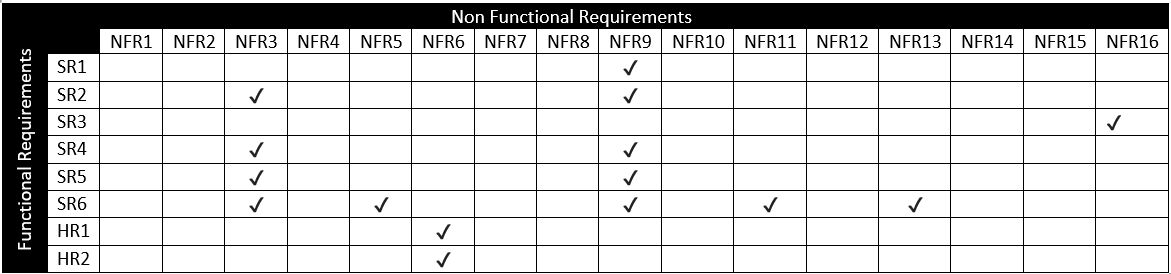
\includegraphics[width=15cm]{images/TraceabilityMatrix.png}
    \caption[]{Traceability Matrix Between Functional Requirements and Non-Functional Requirements}
    \label{fig:figure6}
\end{figure}

\section{System Modes}
N / A - The system itself does not have many relevant states that differ from a base or starting mode, regarding either the user or the data processing. The system should be considered as a continuous data stream, where batches of data are trimmed and processed, all with the goal of passing through the deep learning algorithm. That behavioral state is not subject to change, but rather the environment and context of the learner are what will be iterated on throughout this project.

\section{Plan}

\begin{table}[H]
\centering
\caption{\bf Checkpoints and Deadlines (Subject to Change)}
\begin{tabular}{ |p{6cm}|p{3cm}|p{3cm}|  } 
 \hline
\bf Checkpoint & \bf Date & Status\\
 \hline
Write deep-learner skeleton & Nov 15th & Completed\\
 \hline
Develop phase array & Nov 25th & Completed\\
 \hline
Integrate skeleton with relevant technologies (database, matlab) & Nov 25th & In Progress (Debugging)\\
  \hline
Begin simulation processing: proof of concept & Nov 30th & Completed\\
\hline
Develop LAN Server-Client skeleton & December 10th & Completed\\
\hline
Let learner learn! (and review data to make tweaks and analyze accuracy over time) & Ongoing & N/A\\
\hline
Add exploratory element: close the cycle from learner to simulation & January 30th & In Progress (Debugging)\\
\hline
Analyze benefits of exploratory learning & Ongoing & N/A\\
\hline
Develop server for parallel computing & February 25th & Completed\\
\hline
Stretch goals and maintenance & Remaining dev time & In Progress\\
\hline
\end{tabular}
\end{table}
\subsection{Rationale}
As the machine learner requires the most time to implement (due to training the model), it was decided that the skeleton would need to be created fairly early in our development phase to allow for enough time to fully develop and train the algorithm. This would also identify any potential issues or challenges that would be faced during further implementation of the machine learner, allowing for more time to avoid or plan for those issues. 
\par
Following this, developing the phase array and integrating the deep-learner skeleton are necessary to the advancement of the project. Having the phase array would further aid our understanding of the input/output pairings of the systems, and integrating the skeleton with the relevant technologies would be required to begin producing and using data gathered from simulations to train the deep-learner. 
\par
The next checkpoint was then to develop a server-client socket application that allowed for two way communication on the same network. This was to ensure feasibility in having autonomous communication that would be producing simulation data and passing it to the existing database. This is then followed by the actual training of the machine learner algorithm to ensure the accuracy of the results that were to be produced, alongside analyzing the benefits of exploratory learning. These do not have deadlines as they are conducted indefinitely to continuously enhance and better the model.
\par
Once the machine learner has begun taking data to train itself, the development of the full server-client application began. This saw the server-client application shifting from LAN (requiring devices/clients to be connected to the same network as the server) to WIFI (devices/clients are able to connect to the server from any network). This was completed later as the server-client application served as a means to autonomously conduct simulations and push data to the database, which was doable manually (although less efficient). This means that the machine learner was not entirely dependent on the server-client which allowed the full implementation to be done at a later time.
\par
Lastly, once all essential functionality and requirements have been implemented, the assessment of stretch goals and maintenance would begin.

\section*{References}
We will be referring to documentations provided by Mobilite-Power, however, as of now there are no references to mention.

\bibliographystyle{plainnat}

\bibliography{SRS}

\newpage

\newpage{}
\section*{Appendix --- Reflection}
In order for this project to be successful, there are a plethora of skills required to be obtained. 
\par
One major skill required is the ability to enhance the expertise as well as the familiarity with simulation software such as Matlab. As Mechatronics \& Software students, the fundamentals are present to use Matlab for mathematical related programming (particularly in cases where linear algebra is necessary) but not much experience is present for the case of simulations aside from those specific to certain previous history in physics labs. This will allow the project to be excelled when collecting data to be fed into the machine learning algorithm. One approach to build this skill is to watch / go through online tutorials (particularly from Youtube) where they go over certain practices when performing simulations through Matlab. Another approach to this will be merely practicing the Matlab tools \& features such that familiarity is built with the simulation portions of Matlab. Members of the team will particularly choose the approach of following tutorial videos online as this can be quite helpful as well as done at any time due to its convenience. This will be completed by Eamon. 
\par
Another major skill which will determine the success of this project is the ability to create / program a machine-learning and/or artificial intelligence labeled software. This skill will be pertained to specific individuals in the group but a general understanding of this is required amongst the whole team for the continuous success of the project. One approach to this will be reviewing algorithm research papers online that provide ideas in succeeding in this project. Another method is to reach out to supervisors and industry members when discussing the process of building this as well as request for tips on obtaining the skills. This skill will be one of the most difficult to obtain due to the novelty nature of it in the perspective of the current team. The approach selected to build this skill is by reviewing research papers online as this will include a vast amount of information as well as be convenient; whereas the approach depends on external factors. This will be concluded by Eric.
\par
In addition, the skill of programming standards as well as practices will be a skill necessary to be obtained, particularly to the Mechatronics members as they are not as familiar with the tools \& practices as the Software members. This skill will be approached by discussions during meetings as well as reaching out to other team members (particularly in software) in order to request for their inputs as well as revisions when programming standards are applicable. Another method to build this skill is to review the team’s selected programming standard and use handbooks online that pertain to it as a guide when programming - as practice is built using it, the skill will be developed. The approach selected to build this skill is to reach out to other members with experience in this. This is selected as it is narrowed down particularly to the project as well as builds team communication such that the team is aware of the status of the project. This skill will pertain to Nashit. 
\par
A dire skill that is important for this project is the ability to effectively communicate to other members. This is necessary as when dealing with complex situations and a project such as this, it is impossible for a single individual to succeed given the current constraints. The only option is to work effectively as a team. With all the different components of this project as well as the integration to occur in the future, it is important that the project is communicated in each step. One approach to create this skill is to simply discuss with other members how they would like to do this best as well as asking the right questions. Moreover, it would be effective to be influenced by other practices that can be found online in regards to other successful projects. One key advantage to this team is the industry outreach supervisor; this skill can be developed by discussing this matter with them. This knowledge building will be assigned to Mustafa. The selected choice will be to discuss with other members how they would like to do this best as well as asking the correct questions as well as seeking feedback from team members. 
\par
Finally, another skill required to be obtained is the ability to create the prototype which will fall under embedded systems / hardware programming as well as the electrical abilities for assembly. This is a relatively new skill for all members but will be required to be obtained by certain individuals in the team. This will allow for the prototype to be built effectively as well as performing as per standards. An approach for developing this skill is to watch tutorials online and follow simple projects in which the skills are developed. Another approach is to reach out to colleagues with more expertise in this matter and apply those tips to develop our own personal skills. This knowledge will be acquired by Sam. The selected approach will be to watch tutorials online and follow other projects as this will be convenient as well as allows the ability to follow step-by-step procedures.

\end{document}

